%!TEX root = ../../main.tex
\section{Analysis}

Ever since the world has been interconnected over the Internet, malicious parties have intended to take advantage over their computational resources and digital assets. As technologies improve and the society evolves into a digital world, attacks become more sophisticated, frequent and devastating. It is increasing month by month in an exponential ways, compromising governments and companies systems and data. 

Such has been the risk and consequences of cyber attacks and data breaches that in 2021\cite{10DataBreaches:online}:
\begin{enumerate}
    \item On average a data breach costs up to 8.64 million \ac{USD}.
    \item Global Cybercrime costed over 6 trillion
    \item Businesses fell victim of ransomware every 11 seconds.
    \item Took up to 220 days to contain a data breach, with healthcare industry being the slowest to recover with over 320 days.
    \item  As more users perform remote works cybercriminals keep increasing their attacks over telecommuters and remote access pathways
    \item Properly containing a data breach could have saved up to 1 million \ac{USD} in less than 200 days
    \item More than 8\ac{TB} of data were leaked.
    \item A total of 270 major data breaches occurred, exposing 238 Million of records and 16 billion \ac{USD} per day.
\end{enumerate}

\begin{figure}[h]
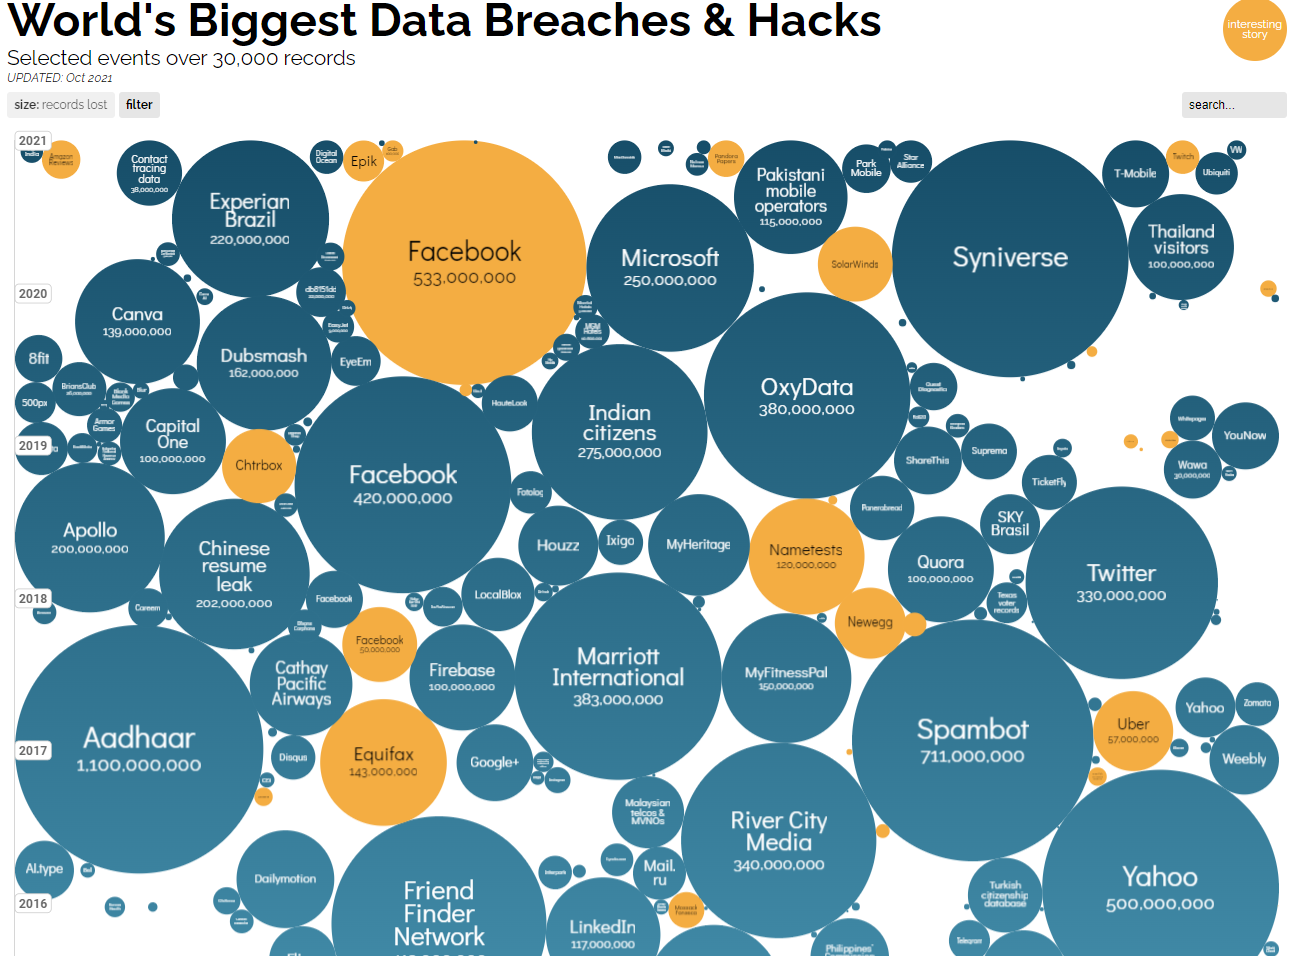
\includegraphics[width=15cm]{img/DataBreach.png}
s\caption{Word's Biggest data breaches and hacks occurred fro 2016 to October 2021  \cite{WorldDataBreach:online}}
\label{fig:worldDataBreach}
\end{figure}
Moreover, in 2021 several Nordic companies were victim of important cyber attacks ,peaking in December 2021\cite{Nordicco81:online}. Affected industries corresponded to the region’s largest industrial, food and  service providing sector.
Affected companies were Vestas, Wind Systems, Amedia, Nortura
and Nordic Choice Hotels

\begin{figure}[h]
\includegraphics[width=15cm]{img/GDPRDataBreach.jpeg}
\centering
\caption{Top-10 GDPR-per-country data breaches notified per EEA jurisdiction from May 2018 to October 2020\cite{Statista:online}}
\end{figure}

It is clear that with the current resources (both human and digital) is impossible to overcome these threats. In addition data has become a vital asset. Companies are now legally liable to protect it and ensure that is properly protected with state of the art technologies. Failing to do that could lead them to bankruptcy or serious fines which in some cases could be of irrecoverable damage, lost of reputation or even catastrophic disasters for the society.


\subsubsection{Hypothesis}
\label{analysis_hyp}

With the implementation of a decentralized system in a Hyperledger Fabric and a chaincode implementing \ac{ERC}-721 standard with \ac{IPFS} network, it will be possible to manage and handle data between organizations in a safer and more secure way. Sharing information and ensuring that the non-repudation\footnote{\input{Footnotes/NonrepudationPrinciple}} principle remains consistent over the network no matter how many parties or users join the infrastructure. 